
\chapter{Cadenas de texto}
\label{strings}
\index{string}

Las cadenas de texto no son como los enteros, los racionales,
y los Booleanos. Una cadena de texto es una {\bf secuencia} de caracteres,
lo cual significa que es una colección ordenada de otros valores,
y algunas veces necesitas acceder algunos de estos valores individuales.
En este capítulo verás cómo analizar, manejar, y modificar cadenas
de texto, y aprenderás sobre algunos de los métodos que las
cadenas de texto proveen. También aprenderás sobre una
herramienta muy poderosa para la manipulación de texto, 
expresiones regulares (también conocidas como ``regexes``).
\index{sequence}
\index{regex}


\section{Una Cadena de Texto es una Secuencia}

\index{sequence}
\index{character}
\index{bracket operator}
\index{operator!bracket}
Una cadena de texto es primariamente una pieza de datos textuales,
pero es técnicamente una secuencia ordenada de caracteres.

Muchos lenguajes de programación te permiten acceder caracteres
individuales de una cadena de texto con índice entre corchetes. 
Esto no es directamente posible en Perl, pero todavía puedes
los caracteres uno a la vez usando el método integrado {\tt comb} 
y el operador corchete:

\begin{verbatim}
> my $cadena = "banana";
banana
> my $cad = $cadena.comb;
(b a n a n a)
> say $cad[1];
a
> say $cad[2];
n
\end{verbatim}
%
El método {\tt comb} en la segunda sentencia divide la cadena de texto
en una lista de caracteres que puedes acceder individualmente con
los corchetes.
\index{comb function and method}
\index{method!comb}
\index{function!comb}
\index{bracket!square}
\index{square bracket operator}
\index{index}
\index{subscript}

La expresión dentro de los corchetes se llama un {\bf índice}
(también llamado subíndice). El índice indica cuales 
caracteres en la secuencia quieres (de ahí el nombre). Pero
puede ser que esto no es lo que esperabas: el artículo con
índice 1 es la segunda letra de la palabra. Para los
científicos de la computación, el índice es usualmente
un desplazo del inicio. Por ejemplo, el índice de la primera 
letra (``b``) es 0, y el índice de la primera ``a`` es 1,
no 2, etcétera.
\index{index!starting at zero}
\index{zero, index starting at}

También podrías extraer una ``rebanada`` de varios caracteres
de una sola vez al usar el operador de rango dentro de los 
corchetes:
\index{slice}

\begin{verbatim}
> say $cad[2..5]
(n a n a)
\end{verbatim}
%
\index{substring}
De nuevo, la subcadena ``nana`` comienza en la tercera letra
de \verb|'banana'|, pero esta letra está indexada 2, y la
sexta letra tiene índice 5.

Aunque esto puede ser útil en ocasiones, esta no es la manera
en la que manejarías cadenas de texto en Perl, el cual tiene
herramientas superiores que son más poderosas y más 
expresivas, así que raramente necesitas usar índices o 
subíndices para acceder caracteres individuales.

También, si existe una necesidad real de acceder y manipular
las letras individuales, haría más sentido almacenarlas en un 
array, pero no hemos hablado sobre arrays todavía, así que
regresaremos a esto más tarde.

\section{Operadores Comunes de Cadenas de Texto}
\index{string!operators}

Perl provee un número de operadores y funciones para el 
manejo de cadenas de texto. Revisemos algunos de los más 
populares.

\subsection{Longitud de una Cadena de Texto}
\index{chars function}
\index{function!chars}
\index{string!length}

La primera cosa que desearíamos saber sobre una cadena de texto 
es su longitud. El método (o función) {\tt chars} devuelve el número de
caracteres de una cadena de texto. Como podemos ver, {\tt chars} puede
usarse con una sintaxis de método o función:
\index{invocation!method}
\index{method invocation}

\begin{verbatim}
> say "banana".chars;   # sintaxis de invocación de método
6
> say chars "banana";   # sintaxis de llamada de función
6
\end{verbatim}
%

\index{Unicode}
\index{grapheme}
Nota que, con el advenimiento de Unicode, la noción 
sobre la longitud de una cadena de texto se ha vuelto 
más complicada que lo era con cadenas de texto ASCII.
Hoy en día, un carácter puede estar compuesto de uno, dos, o 
más bytes. La rutina {\tt chars} devuelve el número de 
caracteres (en el sentido de los grafemas de Unicode, los cuales
son más o menos lo que los humanos perciben como caracteres) dentro
de la cadena, aún cuando algunos caracteres requieren una
codificación de más de 2, 3, o 4 bytes.

Una cadena de texto con una longitud cero (i.e., sin caracteres) se
conoce como una \emph{cadena de texto vacía}.

\subsection{Búsqueda de una Subcadena Dentro de una Cadena de Texto}
\label{find}
\index{index function}
\index{function!index}
\index{substring}

La función integrada {\tt index} usualmente toma dos argumentos,
una cadena de texto y una subcadena (algunas veces conocidas como
la ``paja`` y la ``aguja``), busca la subcadena en la cadena de texto,
y devuelve la posición donde se encuentra la subcadena. Si la subcadena
no se encuentra en la cadena, la función devuelve un valor indefinido:

\begin{verbatim}
> say index "naranja", "ra";
2
> say index "naranja", "je";
Nil
\end{verbatim}
%

\index{offset}
Nuevamente, el índice es un desplazo del inicio de la cadena 
de texto, así que el índice de la primera letra (``n``) es cero,
y el índice de la segunda ``a`` es 3, no 4.
\index{index!starting at zero}

También puedes invocar a {\tt index} con una sintaxis de método:
\begin{verbatim}
> say "naranja".index("ra");
2
\end{verbatim}
%

La función {\tt index} puede tomar un tercer argumento opcional,
un entero que indica donde comenzar la \emph{búsqueda} (y por lo
tanto ignorando en la búsqueda cualquier carácter posterior a
la posición de inicio):

\begin{verbatim}
> say index "naranja", "a", 2;
3
\end{verbatim}
%
Aquí la función {\tt index} comenzó la búsqueda en la ``r`` y encontró 
la posición de la segunda ocurrencia de la subcadena ``a``.
 

\index{function!rindex}
\index{rindex function}
También existe una función {\tt rindex}, la cual realiza la búsqueda
de la subcadena de atrás hacia adelante y devuelve la última posición de 
la subcadena dentro de la cadena de texto:

\begin{verbatim}
> say rindex "naranja", "a";
6
\end{verbatim}
%

Nota que aunque {\tt rindex} inspecciona la cadena de texto
de atrás hacia adelante, la función devuelve una posición
computada desde el inicio de la cadena de texto.

\subsection{Extrayendo una Subcadena de una Cadena de Texto}
\index{substr function or method}
\index{function!substr}
\index{substring}

La función opuesta a {\tt index} es la función (o método) {\tt substr},
la cual, dada una posición inicial y una longitud, extrae una subcadena
de una cadena de texto:

\begin{verbatim}
> say substr "Hacer es la mejor manera de decir.", 0, 5;
Hacer
> say "Hacer es la mejor manera de decir.".substr(12, 5)
mejor
\end{verbatim}
%

\index{chars function}
\index{Unicode}
\index{grapheme}
Nota que, al igual que la función {\tt chars}, la longitud es
expresada en caracteres (o grafemas Unicode), no en bytes.
De igual modo, como puedes observar, los espacios que separan
las palabras dentro de la cadena de texto obviamente cuentan 
como caracteres. El argumento de la longitud es opcional; 
si no se provee, la función {\tt substr} devuelve la subcadena
comenzando en la posición de inicio al final de la cadena de texto:

\begin{verbatim}
> say "Hacer es la mejor manera de decir.".substr(9)
la mejor manera de decir.
\end{verbatim}

Similamente, si el valor de la longitud es muy largo para que 
la subcadena comience en la posición inicial, la función
{\tt substr} devolverá la subcadena comenzando en la posición
inicial hasta el final de la cadena:

\begin{verbatim}
> say substr "banana", 2, 10;
nana
\end{verbatim}

Por supuesto, los parámetros de la posición inicial y la longitud 
no necesitan números literales como en los ejemplos anteriores; puedes
también usar variables (o hasta una expresión o una función que devuelve 
un valor numérico), provisto que la variable o la función pueda ser 
coaccionada en un entero. Pero la posición de inicio debe estar dentro 
del rango de la cadena de texto, y si falla obtienes un error 
{\tt Start argument to substr out of range ...}; por lo tanto
podrías tener que verificarlo en contra de la longitud de la 
cadena de texto con antelación.

También puedes comenzar a contar de atrás hacia adelante con la
siguiente sintaxis:

\begin{verbatim}
> say "I have a dream".substr(*-5)
dream
> say substr "I have a dream", *-5;
dream
\end{verbatim}
%
Aquí, el asterisco * puede considerarse como una representación de la
longitud total de la cadena de texto; \verb|*-5| es por lo tanto la posición
en la cadena de texto cinco caracteres antes del final de la cadena. Así que
\verb|substr(*-5)| devuelve los caracteres desde esa posición hasta el final
de la cadena de texto, i.e., los últimos cinco caracteres de la cadena de
texto.
\index{substr function}
\index{substring}

\subsection{Otras Funciones o Métodos Útiles de Cadenas de Texto}
\index{string!operators}

Esto puede no ser obvio todavía, pero prontamente veremos
que la combinación de las funciones de cadenas de texto que discutimos
más arriab nos dan ya mucho poder para manipular cadenas de texto
más allá de lo que piensas posible en este punto.

Déjanos mencionar brevemente varias funciones adicionales
que pueden ser útiles de vez en cuando.

\subsubsection{flip}

\index{flip function}
\index{function!flip}
La función (o método) {\tt flip} invierte una cadena de texto:

\begin{verbatim}
> say flip "mango";
ognam
\end{verbatim}
%

\subsubsection{split}
\index{split function or method}
\index{function!split}
\index{delimiter}
La función (o método) {\tt split} divide una cadena de texto 
en subcadenas de texto, basado en los delimitadores en l
cadena de texto:

\begin{verbatim}
> say $_ for split "-", "25-12-2016";
> #                 ^ delimitador
25
12
2016
> for "25-12-2016".split("-") -> $val {say $val};
25
12
2016
\end{verbatim}

El delimitador puede ser un solo carácter con comillas como
en el ejemplo más arriba o una cadena de varios caracteres, 
tales como una coma y un espacio en el ejemplo más abajo:

\begin{verbatim}
> .say for split  ", ", "Jan, Feb, Mar";
> #                ^^ delimitador
Jan
Feb
Mar
\end{verbatim}

Recuerda que \verb|.say| es un atajo para \verb|$_.say|.

Por defecto, los delimitadores no aparecen en la salida producida por 
la función (o método) {\tt split}, pero este comportamiento puede 
cambiarse con el uso de {\tt adverbio} apropiado. Un adverbio es básicamente
un argumento nombrado de una función que modifica la manera en la 
función se comporta. Por ejemplo, el adverbio {\tt :v} (valores)
le dice a {\tt split} que también devuelva el valor del delimitador:
\index{adverb}
\index{:v adverb}

\begin{verbatim}
> .perl.say for split  ', ', "Jan, Feb, Mar", :v;
"Jan"
", "
"Feb"
", "
"Mar"
\end{verbatim}

Los otros adverbios que pueden usarse en este contexto son {\tt :k} (claves), 
{\tt :kv} (claves y valores), y {\tt :p} (pares). Su significados detallados pueden
encontrarse en la documentación para {\tt split}
(\url{https://docs.perl6.org/routine/split}). El adverbio {\tt skip-empty}
remueve las partes vacías de la lista de resultados.

La función {\tt split} pueden también usarse un \emph{patrón} 
de expresión regular como un delimitador, y esto puede hacerla
mucho más poderosa. Estudiaremos expresiones regulares más adelante
en este capítulo.
\index{regular expression}
\index{regex}

\subsubsection{Concatenación de Cadenas de Texto}

\index{concatenate operator}
\index{string!concatenation}
\index{string concatenation}

El operador \verb|~| concatena dos cadenas de texto y forma una:

\begin{verbatim}
> say "ban" ~ "ana";
banana
\end{verbatim}
%

Puedes tener cadenas de varias ocurrencias de este operador
para concatenar más de dos cadenas:

\begin{verbatim}
> say "ba" ~ "na" ~ "na";
banana
\end{verbatim}
%

Si se usa como un operador prefijo unario,
\verb|~| transforma su argumento en una cadena de texto:
\index{stringify operator}
\index{stringification}

\begin{verbatim}
> say (~42).WHAT;
(Str)
\end{verbatim}
%

\subsubsection{Separando en Palabras}

\index{words function or method}
La función {\tt words} devuelve una lista de palabras
que componen la cadena de texto:

\begin{verbatim}
> say "I have a dream".words.perl;
("I", "have", "a", "dream").Seq
> .say for "I have a dream".words;
I
have
a
dream
\end{verbatim}
%

\subsubsection{join}

\index{join function or method}
\index{function!join}
La función {\tt join} toma un argumento separador y una lista
de cadenas de texto como argumentos; la función las intercala
con el separador, concatena todo en una sola cadena de texto, y 
devuelve la cadena de texto resultante.

Este ejemplo ilustra el uso de las funciones (o métodos) 
{\tt words} y {\tt join}:

\begin{verbatim}
say 'I have a dream'.words.join('|');    # -> I|have|a|dream
say join ";", words "I have a dream";    # -> I;have;a;dream
\end{verbatim}
%

\index{words function or method}
En ambos casos, {\tt words} primero divide la cadena original
en una lista de palabras,  {\tt splits} sutura los artículos
de esta lista y los devuelve en una nueva cadena de texto 
intercalados con el separador.

\subsubsection{Conversión a Minúscula y a Mayúscula}
\index{lc function or method} 
\index{lower case!lc function}
\index{uc function or method}
\index{tc function or method}
\index{upper case}
\index{lower case}
\index{title case}
\index{case!upper}
\index{case!lower}
\index{case!title}

Las rutinas {\tt lc} y {\tt uc} devuelven respectivamente
una versión en minúscula y una versión mayúscula de sus 
argumentos. También está la función {\tt tc} la cual devuelve
su argumento con la primera letra en mayúscula:

\begin{verbatim}
say lc "Abril";    # -> april
say "Abril".lc;    # -> april
say uc "abril";    # -> APRIL
say tc "abril";    # -> April
\end{verbatim}

\index{eq, string equality operator}
Recuerda que el operador {\tt eq} chequea la igualdad de dos 
cadenas de texto.

\section{Recorrido de una Cadena con un bucle {\tt while} o {\tt for}}
\label{stringtraversal}
\index{traversal}
\index{loop!traversal}
\index{for loop}
\index{loop!for}
\index{statement!for}
\index{index function}
\index{while loop}

Muchas computaciones involucran el procesamiento de una
cadena de texto una carácter a la vez. Usualmente ellas
comienzan al principio, seleccionan cada carácter en turno,
hacen algo con dicho carácter, y continúan hasta el final.
Este patrón de procesamiento se conoce como {\bf recorrido}. 
Una manera de escribir un recorrido es con un bucle {\tt while}
y la función {\tt index}:
\index{while loop}
\index{index}

\begin{verbatim}
my $indice = 0;
my $fruta = "banana";
while $indice < $fruta.chars { 
    my $letra = substr $fruta, $indice, 1; 
    say $letra; 
    $indice++;
}
\end{verbatim}
%

Esto imprimirá cada letra, una a la vez:
\begin{verbatim}
b
a
n
a
n
a
\end{verbatim}
%
Este bucle recorre la cadena de texto y muestra cada letra
en un línea por si misma. La condición del bucle es 
{\tt \$indice < \$fruta.chars},
así que cuando {\tt \$indice} es igual a la longitud de
la cadena de texto, la condición es falsa, y el cuerpo del
bucle no se ejecuta. En otras palabras, el bucle para cuando
{\tt \$indice} es la longitud de la cadena de texto menos 
uno, lo cual corresponde al último carácter de la cadena 
de texto.

Como ejercicio, escribe una función que toma una cadena de 
texto como un argumento y muestra las letras de atrás hacia
adelante, una por línea. Hazlo por lo menos una vez sin utilizar
la función {\tt flip}. Solución: \ref{sol_stringtraversal}

Otra forma de escribir un recorrido es con un bucle {\tt for}:
\index{for loop}
\index{comb function and method}

\begin{verbatim}
my $fruta = "banana";
for $fruta.comb -> $letra {
    say $letra
}
\end{verbatim}
%

Cada vez a través del bucle, el siguiente carácter en la
cadena de texto es asignado a la variable {\tt \$letra}.
El bucle continúa hasta que no hayan más caracteres.

El bucle podría también usar la función {\tt substr}:
\index{index function}

\begin{verbatim}
for 0..$fruta.chars - 1 -> $indice {
    say substr $fruta, $indice, 1;
}
\end{verbatim}
%

\index{concatenation}
\index{abecedarian}
\index{aphabetic order}
\index{McCloskey, Robert}

El siguiente ejemplo muestra cómo usar concatenación y
un bucle {\tt for} para genera una serie de abecedario (
es decir, en orden alfabético). En el libro 
{\em Make Way for Ducklings} de McCloskey, los nombres de los
patitos son Jack, Kack, Lack, Mack, Nack, Ouack, Pack, y Quack. 
Este bucle podría muestra estos nombres en orden:

\begin{verbatim}
my $sufijo = 'ack';
for 'J'..'Q' -> $letra {
    say $letra ~ $sufijo;
}
\end{verbatim}
%
La salida es:

\begin{verbatim}
Jack
Kack
Lack
Mack
Nack
Oack
Pack
Qack
\end{verbatim}
%
Por supuesto, esto no es del todo correcto dado que ``Ouack'' y 
``Quack'' están mal escritos. Como ejercicio, modifica el programa
para arreglar este error. Solución: \ref{sol_ducklings}.


\section{Bucles y Conteo}
\label{counter}
\index{counter}
\index{counting and looping}
\index{looping and counting}
\index{looping!with strings}

El siguiente programa cuenta el número de veces que 
la letra ``a`` aparece en una cadena de texto:
\index{comb function and method}

\begin{verbatim}
my $palabra = 'banana';
my $conteo = 0;
for $palabra.comb -> $letra {
    $conteo++ if $letra eq 'a';
}
say $conteo;              # -> 3
\end{verbatim}
%

\index{counter}
Este programa demuestra otro patrón de la computación 
llamado {\bf contador}. La variable \verb|$conteo| se inicializa
a 0 y después se incrementa por uno cada vez que se encuentra
una ``a``. Cuando el bucle termina, \verb|$conteo| contiene
el resultado---el número total de ocurrencias de la letra ``a``.
\index{incrementation}

\index{encapsulation}
Como ejercicio, encapsula este código en una subrutina llamada
{\tt contar}, y generalízala para que acepte una cadena de texto 
y la letra a contar como argumentos. Solución: \ref{sol_count_letters}.
\label{count_letters}

\section{Expresiones Regulares (Regexes)}
\label{regex}
\index{regex}
\index{regular expression}

Las funciones y los métodos de cadenas de texto que hemos visto
hasta ahora son realmente poderosos, y pueden usarse para un 
sin número de operaciones relacionadas con la 
manipulación de cadenas de texto. Pero supón que quieres extraer
de la cadena ``yellow submarine`` cualquier letra después
de la letra ``l`` y antes de la letra ``w``. Este tipo de 
``búsqueda difusa`` puede hacerse con un bucle, pero no 
es práctico. Puedes hacerlo como un ejercicio si deseas,
pero debo advertirte: es algo delicado y difícil. Aún si 
no lo haces, la solución puede interesarte: 
ver Subsección\ref{sol_regex_loop}. 
\label{regex_loop}

Si agregas otra condición, por ejemplo que esta letra 
debería extraerse o \emph{capturarse} (i.e. almacenada para 
uso futuro) solo si el resto de la cadena de texto contiene
la subcadena ``rin``, esto comienza a ser algo tedioso. También,
cualquier cambio a los requerimientos conduce a que tengamos
que hacer una reescritura substancial o hasta refactorizar
el código completamente.

Para este tipo de trabajo, una {\bf expresión regular} 
o un {\bf regex} es una herramienta mucha más poderosa
y expresiva. La siguiente es una manera de extraer letras usando
el criterio descrito anteriormente: 


\begin{verbatim}
> my $cadena = "yellow submarine";
yellow submarine
> say ~$0 if $cadena ~~ / l (.) w .*? rin /;
o
\end{verbatim}

No te preocupes si no entiendes este ejemplo;
afortunadamente todo se aclarará muy pronto.

\index{operator!smart match}
\index{smart match operator}
El operador \verb|~~| se conoce como el operador de coincidencia
inteligente. Es un operador de relación muy poderoso que puede
usarse para tareas de comparación más avanzadas. En este caso, 
el operador chequea si la variable {\tt \$cadena} a su izquierda
``coincide`` con la expresión a su derecha, i.e., como una 
primera aproximación, si la expresión a su derecha describe la 
cadena de texto (o parte de la misma).

\index{pattern}
La parte \verb|/ l (.) w .*? rin /| se llama un patrón de regex y puede
describirse así: la letra ``l``, seguida por cualquier otro carácter (el
punto) para ser capturado (gracias a los paréntesis), seguida por la
letra ``w``, seguida por un número no específico de caracteres,
seguida por la subcadena ``rin``. ¡Uff! ¡Todo esto en una sola línea
de código! Bien poderoso, no lo crees? Si la cadena de texto coincide 
con el patrón, entonces la coincidencia devolverá un valor verdadero y 
la variable \verb|$0| será poblada con el carácter a ser capturado---
la letra ``o`` en este caso.
\index{capture}

A menos que sea especificado (veremos cómo hacerlo luego),
los espacios en blanco no son significantes dentro de un 
patrón de regex. Así que puedes agregar espacios dentro de una patrón
para separar sus piezas y hacer tus intenciones más claras.

La mayor parte de este capítulo discutirá los fundamentos de 
la construcción de tales patrones de regex y cómo usarlos. 
Pero el concepto de los regexes es tan crucial en Perl que 
dedicaremos un capítulo completo a este tema y otros asuntos
relacionados (Capítulo~\ref{regex_grammars}).

La noción de la expresiones regulares es originalmente un 
concepto procedente de las teoría de lenguajes formales. 
El primer uso de expresiones regulares en la computación fue 
en las utilidades Unix, algunas de las cuales permanecen en 
extenso uso hoy en día, tales como {\tt grep}, creada por Ken Thomson en 1973,
{\tt sed} (ca. 1974), y {\tt awk}, desarrollada años más tarde (en 1977)
por  Aho, Weinberger, and Kernighan. 
Las versiones anteriores del lenguaje Perl en el decenio del 1980
incluían una versión extendida de las expresiones regulares, que 
ha sido desde tal entonces imitada por muchos otros lenguajes de
programación. La diferencia, no obstante, es que las expresiones
regulares están profundamente arraigadas en el núcleo del lenguaje
Perl, mientras que los otros lenguajes las han adoptado como un
add-on o plug-in, usualmente basado o derivado de una librería 
conocida como Expresiones Regulares Compatible con Perl (PCRE 
por sus siglas en inglés).
\index{awk}
\index{grep}
\index{Thomson, Ken}
\index{sed}
\index{Aho, Alfred}
\index{Weinberger, Peter}
\index{Kernighan, Brian}
\index{PCRE (Perl Compatible Regular Expressions)}
\index{Perl Compatible Regular Expressions (PCRE)}

Las expresiones regulares de Perl han extendido estas nociones
tanto que tienen muy poco que ver con el concepto original de 
teoría de lenguaje , y por lo tanto se ha considerado 
apropiado parar de llamarlas \emph{expresiones regulares}
y hablar de \emph{regexes}, i.e., un tipo de sub-lenguaje
de coincidencia de patrón que funciona de manera similar
a las expresiones regulares.

\section{Uso de los Regexes}
\label{using_regexes}
\index{smart match operator}

Una manera simple de usar un regex es utilizar el operador
de coincidencia inteligente \verb|~~|:
\index{smart match operator}
\index{operator!smart match}

\begin{verbatim}
say "Coincidió" if "abcdef" ~~ / bc.e /;     # -> Coincidió
\end{verbatim}
%

Aquí, el operador de coincidencia inteligente compara la 
cadena de texto ``abcdef`` con el patrón $/bc.e/$ y reporta
una comparación exitosa dado que, en este caso, ``bc`` en la
cadena coincide con la parte $bc$ del patrón, el punto en el
patrón coincide con cualquier carácter en la cadena (
y coincidió en este caso con $d$) y, finalmente, la $e$ de la
cadena coincide con la $e$ en el patrón.

\index{stringify operator}
\index{matched string}
La parte de la cadena que coincidió es almacenada en la variable
\verb|$/| que representa el {\bf objeto coincidencia}, el cual
podemos convertir en una cadena de texto con el operador \verb|~|.
Podemos hacer un buen uso de esto para visualizar la parte de la
cadena que coincidió con el patrón de regex:

\begin{verbatim}
say ~$/ if "abcdef" ~~ / bc.e /;           # -> bcde
\end{verbatim}
%


\index{backtracking}

El proceso de coincidencia podría describirse en la siguiente
forma (pero ten presente que esto una simplificación): busca en 
la cadena de texto (desde izquierda a derecha) un carácter que 
coincide con el primer átomo (i.e., el primer artículo de 
coincidencia) del patrón; cuando se encuentra, busca si el segundo
carácter puede coincidir el segundo átomo del patrón, etc. Si
se usa el patrón entero, entonces el regex fue exitoso. Si falla
durante el proceso, comienza nuevamente desde la posición 
inmediatamente después del punto de coincidencia inicial. (
Esto se conoce como {\bf vuelta atrás} o \emph{backtracking} en inglés).
Y se repite hasta que uno de los siguientes casos ocurra:

\begin{itemize}
\item Hay una coincidencia exitosa. En este caso, el proceso
finaliza y se reporta éxito. 
\item La cadena de texto ha sido agotada sin encontrar la 
coincidencia. En este caso, el regex falla.
\end{itemize}

Examinemos un ejemplo de vuelta atrás:
\begin{verbatim}
say "Coincidió" if "abcabcdef" ~~ / bc.e /;  # -> Coincidió
\end{verbatim}
%
% abcabcdef
%  bc.e 
% After bactracking
% abcabcdef
%     bc.e 

\index{backtracking}
En este ejemplo, el motor de regex comienza a coincidir 
``bca`` con $bc.$, pero el atento coincidencia inicial falla,
porque la siguiente letra en la cadena de texto, ``b``, no
coincide con la ``e```del patrón. El motor de regex da vuelta
atrás e inicia la búsqueda nuevamente desde la tercera letra (``c``)
de la cadena. Comienza una nueva coincidencia en la quinta letra de
la cadena (la segunda ``b``), logra coincidir exitosamente con
``bcde`` y sale con un estado exitoso (sin buscar ninguna otra
coincidencia).

Si la cadena de texto a analizar está contenida en la 
variable tópico \verb|$_|, entonces el operador de coincidencia
inteligente es implícito y la sintaxis es aún más simple:
\index{topical variable}

\begin{verbatim}
for 'abcdef' {                                # $_ ahora contiene a 'abcdef'
    say "Coincidió" if / cd.f /;              # -> Coincidió
}
\end{verbatim}
%

También puedes usar una sintaxis de invocación de método:
\index{match method}
\index{method!match}
\index{invocation!method}
\index{method invocation}
\begin{verbatim}
say "Coincidió" if "abcdef".match(/ b.d.f /); # -> Coincidió
\end{verbatim}
%

En todos los casos que hemos visto hasta ahora, usamos 
directamente un patrón dentro de un par de delimitadores de barra
oblicua $/$. Podemos utilizar otros delimitadores si precedemos
nuestro patrón con la letra ``m``:
\index{regex!pattern delimiter}

\begin{verbatim}
say "Coincidió" if "abcdef" ~~ m{ bc.e };     # -> Coincidió
\end{verbatim}
%

o:
\begin{verbatim}
say "Coincidió" if "abcdef" ~~ m! bc.e !;     # -> Coincidió
\end{verbatim}
%

El operador ``m`` no altera la manera en que un regex funciona;
solo hace posible el uso de otros delimitadores (además de las
barras oblicuas). Dicho diferentemente, el prefijo ``m`` es la
manera estándar de introducir un patrón, pero es implícito y 
puede omitirse cuando el patrón es delimitado por barras oblicuas.
Es probablemente mejor usar barras oblicuas, porque es lo que la
gente comúnmente utiliza y reconoce inmediatamente, y usar otros
delimitadores solo cuando el patrón de regex contiene barras
oblicuas.

Un patrón puede también almacenarse en una variable (o, más
precisamente, en un objeto regex), usando el operador $rx//$:
\index{rx regex operator}

\begin{verbatim}
my $regex = rx/c..f/;
say "Coincidió" if 'abcdef' ~~ $regex;        # -> Coincidió
\end{verbatim}
%


\section{Cómo Construir tus Patrones Regex}
\label{pattern}
\index{pattern}

Es ahora tiempo para estudiar los componentes básicos de 
un patrón regex.

\subsection{Coincidencia Literal}
\index{literal matching}

Como posiblemente ya has notado, el caso más simple de un
patrón de regex es una cadena de texto constante. Coincidir
una cadena de texto en contra de tal regex es más o menos 
equivalente a una búsqueda de esa cadena con la función 
{\tt index}:
\index{index function}

\begin{verbatim}
my $cadena = "superlative";
say "$cadena contiene 'perl'." if $cadena ~~ /perl/;
                               # -> superlative contiene 'perl'.
\end{verbatim}
%

\index{index}
\index{contains}
Sin embargo nota que, para tales coincidencias literales, 
la función {\tt index} discutida anteriormente será probablemente
más eficiente que un regex con cadenas de texto largas. 
El método {\tt contains}, el cual devuelve verdadero si su
argumento es una subcadena de su invocante, es también probablemente
más rápido.
\index{invocant}

Los caracteres alfanuméricos y la raya baja \verb|_| son coincidencias
literales. Todos los otros caracteres deben escaparse con una barra
invertida (por ejemplo \verb|\?| para coincidir con un signo de interrogación
derecho) o incluirse dentro de comillas:

\begin{verbatim}
say "Éxito" if 'nombre@org.uk' ~~ / nombre@or /;      # Falla en la compilación
say "Éxito" if 'nombre@org.uk' ~~ / 'nombre@or' /;    # -> Éxito
say "Éxito" if 'nombre@org.uk' ~~ / nombre\@or/ ;     # -> Éxito
say "Éxito" if 'nombre@org.uk' ~~ / nombre '@' org /; # -> Éxito
\end{verbatim}
%


\subsection{Comodines y Categorías de Caracteres}
\index{character class}

Los regexes no serían muy útiles si solo pudieran hacer 
coincidencia literal. Ahora nos acercamos a las partes más 
interesantes.

En un patrón de regex, algunos símbolos pueden coincidir no
con un carácter específico, sino con una familia de caracteres,
tales como letras, dígitos, etc. Estos símbolos se conocen como
categorías de clases.

Ya hemos visto que el punto es un tipo de comodín que
coincide con un solo carácter de la cadena de texto a
coincidir:
\index{wildcard character}

\begin{verbatim}
my $cadena = "superlative";
say "$cadena contiene 'pe.l'." if $cadena ~~ / pe . l /;
                       # -> superlative contiene 'pe.l'.
\end{verbatim}
%

El ejemplo más arriba ilustra otra característica
de los regexes: los espacios en blanco son usualmente
no significantes dentro de los patrones de regex 
(a menos que se especifiquen con el adverbio 
$:s$ o $:sigspace$, como veremos más adelante).
\index{whitespace in regexes}

Hay categorías de caracteres predefinidas de la forma \verb|\w|.
Su negación se escribe con una letra en mayúscula, \verb|\W|.
El carácter de palabra \verb|\w| coincide con un solo carácter 
alfanumérico (i.e., entre los caracteres alfanuméricos, dígitos,
y el carácter \verb|_|). \verb|\W| coincidirá cualquier otra carácter
que no sea un carácter de palabra. Nota, sin embargo, que Perl
es compatible con Unicode y que, por ejemplo, letras del alfabeto
griego o cirílico o dígitos tailandenses coincidirán con \verb|\w|:

\begin{verbatim}
say "Coincidió" if 'abcδ' ~~ / ab\w\w /;  # -> Coincidió
\end{verbatim}
%

En este ejemplo, las cadenas de texto coincidieron porque, de 
acuerdo al estándar Unicode, \verb|δ| (``\textsc{Greek small letter delta}'')
es una letra y por lo tanto pertenece a la categoría de  
clase \verb|\w|.

Otras categorías de clase incluyen:
\begin{itemize}
\item \verb|\d| (dígitos) y \verb|\D| (cualquier carácter menos un dígito)
\item \verb|\s| (espacio en blanco) y \verb|\S| (cualquier carácter menos un espacio en blanco)
\item \verb|\n| (línea nueva) y \verb|\N| (cualquier carácter menos una línea nueva).
\end{itemize}

\begin{verbatim}
say ~$/ if 'Bond 007' ~~ /\w\D\s\d\d\d/;  # -> "nd 007"
\end{verbatim}
%

Aquí, coincidimos con ''nd 007'', porque encontramos un
carácter de palabra (''n''), seguido por un un carácter que 
no es un dígito (``d``), seguido por un espacio en blanco,
seguido por tres dígitos.

También puedes especificar tus propias categorías de caracteres
al insertar entre \verb|<[ ]>| cualquier número de caracteres
individuales y rangos de caracteres (expresado con dos puntos 
entre los puntos extremos), con o sin espacio en blanco. Por 
ejemplo, una categoría de caracteres para dígitos hexadecimales
podría lucir así:
\begin{verbatim}
<[0..9 a..f A..F]>
\end{verbatim}

Puedes negar cualquier categoría de caracteres al insertar un 
``-`` después de la comilla angular izquierda. Por ejemplo,
una cuerda no es un entero hexadecimal válido si contiene
cualquier carácter que no está en \verb'<[0..9a..fA..F]>', i.e.m
cualquier carácter que coincide con la categoría de caracteres
de hexadecimales negada:
\index{negated character class}

\begin{verbatim}
say "No un número hex" if $cadena ~~ /<-[0..9 a..f A..F]>/;
\end{verbatim}

Por favor nota que generalmente no tienes que escapar
caracteres que no son alfanuméricos en tus categorías de 
caracteres:

\begin{verbatim}
say ~$/  if "-17.5" ~~ /(<[\d.-]>+)/; # -> -17.5
\end{verbatim}

En este ejemplo, usamos el cuantificador ''+'' que discutiremos
en la siguiente sección, pero el punto aquí es que no necesitas
escapar el punto y la barra oblicua dentro de la definición de
categoría de caracteres.

\subsection{Cuantificadores}
\index{quantifier}

Un cuantificador hace que un átomo\footnote{
La palabra \emph{átomo} se refiere a un carácter 
individual o varios caracteres u otros átomos
agrupados juntos (por un conjunto de paréntesis 
o corchetes).} precedente coincida no solamente 
una vez, sino un específico o variable número de
veces. Por ejemplo, \verb|a+| coincide una o más
caracteres ''a''. En el siguiente código, \verb|\d+| 
coincide con uno o más dígitos (tres dígitos en este caso):

\begin{verbatim}
say ~$/ if 'Bond 007' ~~ /\w\D\s\d+/;  # -> "nd 007"
\end{verbatim}
%

Los cuantificadores predefinidos incluyen:
\begin{itemize}
\item $+$: una o más veces;
\item $*$: cero o más veces;
\item $?$: cero o un coincidencia.
\end{itemize}

\index{greedy quantifier}
\index{quantifier!greedy}
Los cuantificadores $+$ and $*$ se dice que son \emph{voraces}
(o \emph{greedy} en inglés), lo que significa que ellos
coinciden con tantos caracteres como sea posible. Por ejemplo:

\begin{verbatim}
say ~$/ if 'aabaababa' ~~ / .+ b /;     # -> aabaabab
\end{verbatim}
%

Aquí, \verb|.+| coincide con tanto de la cadena de texto
como sea posible, mientras que es capaz de coincidir con
la final ''b''. Usualmente esto es lo que deseas, pero 
siempre. Quizás tu intención era coincidir con todas las letras
hasta la primera ``b``. En tales casos, usarías las versiones
\emph{frugales} (no voraz) de estos cuantificadores, los cuales
se obtienen al  precederlos con un signo interrogación derecho:
$+?$ y $*?$. Un cuantificador frugal coincidirá con tanto como
sea posible para que el regex sea exitoso pero no más que eso.
Para coincidir con todas las letras hasta la primera $b$, podrías
usar:
\index{frugal quantifier}
\index{quantifier!frugal}

\begin{verbatim}
say ~$/ if 'aabaababa' ~~ / .+? b /;     # -> aab
\end{verbatim}
%

También podrías especificar un rango ({\tt min..max}) para el 
número de veces que un átomo debe coincidir. Por ejemplo, para 
coincidir con un entero menor que 1,000:
\index{range quantifier}
\index{quantifier!range}

\begin{verbatim}
say 'Es un número < 1,000' if $cadena ~~ / ^ \d ** 1..3 $ /;
\end{verbatim}
%

Esto coincide con uno a tres dígitos. Los caracteres \verb|^|
y \verb|$| son anclas que representan el inicio y el final
de la cadena de texto y los discutiremos en la siguiente
sección.

Para coincidir un número exacto de veces, solo reemplaza el 
rango con un número individual:
\index{quantifier!exact number of times}

\begin{verbatim}
say 'Es un número de 3 dígitos' if $num ~~ / ^ \d ** 3 $ /;
\end{verbatim}
%

\subsection{Anclas y Aserciones}
\index{anchor}
\index{regex!anchor}
\index{assertion}

Algunas veces, coincidir con una subcadena no es suficientemente
bueno; quieres coincidir con la cadena de texto completa, 
o quieres que la coincidencia ocurra al comienzo o al final de la cadena,
o en algún lugar específico dentro de la cadena. Las anclas y las 
aserciones hacen posible especificar donde la coincidencia debe
ocurrir. Necesitan coincidir exitosamente para que el regex completo
para tener éxito, pero no consumen los caracteres mientras la 
coincidencia ocurre.

\subsubsection{Anclas}

\index{start of string anchor}
\index{end of string anchor}
\index{anchor!start of string}
\index{anchor!end of string}

The most commonly used anchors are the \verb'^' start of 
string and \verb'$' end of string anchors:

\begin{verbatim}
my $string = "superlative";
say "$string starts with 'perl'" if $string ~~ /^perl/; # (No output)
say "$string ends with 'perl'" if $string ~~ /perl$/;   # (No output)
say "$string equals 'perl'" if $string ~~ /^perl$/;     # (No output)
\end{verbatim}

All three regexes above fail because, even though 
\verb|$string| contains the ``perl'' substring, the 
substring is neither at the start, nor at the end of 
the string.

\index{start of line anchor}
\index{end of line anchor}
\index{anchor!start of line}
\index{anchor!end of line}
In the event that you are handling multiline strings, you might 
also use the \verb'^^' start of line and \verb|$$| end of line anchors.

There are some other useful anchors, such as the \verb'<<' 
start of word (or word left boundary) and \verb'>>' end 
of word (or word right boundary) anchors.
\index{anchor!word boundary}
\index{anchor!start of word}
\index{anchor!end of word}
\index{anchor!left word boundary}
\index{anchor!right word boundary}

\subsubsection{Look-Around Assertions}

\index{look-around assertion}
\index{assertion!look around}
\index{assertion!look before}
\index{assertion!look after}

\emph{Look-around assertions} make it possible to 
specify more complex rules: for example, match ``foo'', 
but only if preceded (or followed) by ``bar'' (or not 
preceded or not followed by ``bar''):

\begin{verbatim}
say "foobar" ~~ /foo <?before bar>/; # -> foo (lookahead assertion)
say "foobaz" ~~ /foo <?before bar>/; # -> Nil (regex failed)
say "foobar" ~~ /<?after foo> bar/;  # -> bar (lookbehind assertion)
\end{verbatim}
%
\index{negative look-around assertion}
\index{assertion!negative look around}
Using an exclamation mark instead of a question mark transforms 
these look-around assertion into negative assertions. For example:

\begin{verbatim}
say "foobar" ~~ /foo <!before baz>/; # -> foo 
say "foobaz" ~~ /foo <!before baz>/; # -> Nil (regex failed)
say "foobar" ~~ /<!after foo> bar/;  # -> Nil (regex failed)
\end{verbatim}
%
I assume that the examples above are rather clear. Look into the 
documentation 
(\url{https://docs.perl6.org/language/regexes#Look-around_assertions}) 
if you need further details. 

\subsubsection{Code Assertions}

You can also include a code assertion \verb'<?{...}>', which 
will match if the code block returns a true value:
\index{code assertion}
\index{assertion!code}

\begin{verbatim}
> say ~$/ if /\d\d <?{$/ == 42}>/ for <A12 B34 C42 D50>;
42
\end{verbatim}

\index{assertion!negative code}
A negative code assertion \verb'<!{...}>' will 
match unless the code block returns a true value:
\begin{verbatim}
> say ~$/ if /\d\d <!{$/ == 42}>/ for <A12 B34 C42 D50>
12
34
50
\end{verbatim}

Code assertions are useful to specify conditions that 
cannot easily be expressed as regexes. 

They can also be used to display something, for example 
for the purpose of debugging a regex by printing out 
information about partial matches:

\begin{verbatim}
> say "Matched $/" if "A12B34D50" ~~ /(\D) <?{ say ~$0}> \d\d$/;
A
B
D
Matched D50
\end{verbatim}

The output shows the various attempted matches that 
failed (``A'' and ``B'') before the backtracking 
process ultimately led to success (``D50'' at the end 
of the string).

However, code assertions are in fact rarely needed for 
such simple cases, because you can very often just add 
a simple code block for the same purpose:
%
\begin{verbatim}
> say "Matched $/" if "A12B34D50" ~~ /(\D) { say ~$0} \d\d$/;
\end{verbatim}
This code produces the same output, and there is no need 
to worry about whether the block returns a true value.


\subsection{Alternation}
\index{alternation}

Alternations are used to match one of several alternatives.

For example, to check whether a string represents one of the 
three base image colors (in JPEG and some other image formats), 
you might use:

\begin{verbatim}
say 'Is a JPEG color' if $string ~~ /^ [ red | green | blue ] $/;
\end{verbatim}
%

\index{first-match alternation}
There are two forms of alternations. First-match alternation 
uses the \verb'||' operator and stops on the first alternative 
that matches the pattern:

\begin{verbatim}
say ~$/ if "abcdef" ~~ /ab || abcde/;       # -> ab
\end{verbatim}
%

Here, the pattern matches ``ab'', without trying to match 
any further, although there would be an arguably ``better'' 
(i.e., longer) match with the other alternative. When using 
this type of alternation, you have to think carefully about 
the order in which you put the various alternatives, 
depending on what you need to do.

\index{longest-match alternation}
The longest-match alternation uses the \verb'|' operator 
and will try all the alternatives and match the longest one:

\begin{verbatim}
say ~$/ if "abcdef" ~~ /ab | abcde/;        # -> abcde
\end{verbatim}
%

Beware, though, that this will work as explained only if 
the alternative matches all start on the same position 
within the string:

\begin{verbatim}
say ~$/ if "abcdef" ~~ /ab |  bcde/;        # -> ab
\end{verbatim}
%

Here, the match on the leftmost position wins (this is 
a general rule with regexes).


\subsection{Grouping and Capturing}
\index{grouping}
\index{capturing}
\index{parentheses!grouping and capturing}
\index{regex!parentheses versus brackets}
\index{bracket!square}
\index{square bracket}
\index{square bracket operator}

Parentheses and square brackets can be used to group 
things together or to override precedence:

\begin{verbatim}
/ a || bc /      # matches 'a' or 'bc'
/ ( a || b ) c / # matches 'ac' or 'bc'
/ [ a || b ] c / # Same: matches 'ac' or 'bc', non-capturing grouping
/ a b+ /         # Matches an 'a' followed by one or more 'b's
/ (a b)+ /       # Matches one or more sequences of 'ab'
/ [a b]+ /       # Matches one or more sequences of 'ab', non-capturing
/ (a || b)+ /    # Matches a sequence of 'a's and 'b's(at least one)
\end{verbatim}
%

\index{capture}
The difference between parentheses and square brackets is 
that parentheses don't just group things together, 
they also capture data: they make the string matched within 
the parentheses available as a special variable (and also 
as an element of the resulting match object):

\begin{verbatim}
my $str =  'number 42';
say "The number is $0" if $str ~~ /number\s+ (\d+) /;  # -> The number is 42
\end{verbatim}
%

\index{numbered capture}
\index{capture!numbered}
Here, the pattern matched the \verb'$str' string and the 
part of the pattern within parentheses was captured into 
the \verb'$0' special variable. Where there are several 
parenthesized groups, they are captured into variables 
named \verb'$0', \verb'$1',  \verb'$2', etc. (from 
left to right counting the open parentheses):

\begin{verbatim}
say "$0 $1 $2" if "abcde" ~~ /(a) b (c) d (e)/;       # -> a c e
# or: say "$/[0..2]" if "abcde" ~~ /(a) b (c) d (e)/; # -> a c e
\end{verbatim}
%

The \verb'$0', \verb'$1', etc. variables are actually a 
shorthand for \verb'$/[0]', \verb'$/[1]', the first and 
second items of the matched 
object in list context, so that printing  
\verb'"The number is $/[0]"' would have had the same 
effect. 

As noted, the parentheses perform two roles in regexes: 
they group regex elements and they capture what is matched 
by the subregex within parentheses. If you want only the 
grouping behavior, use square brackets
\verb'[ ... ]' instead:

\begin{verbatim}
say ~$0 if 'cacbcd' ~~ / [a||b] (c.) /;   # -> cb
\end{verbatim}
%

Using square brackets when there is no need to capture 
text has the advantage of not cluttering the \verb'$0', 
\verb'$1', \verb'$2', etc. variables, and it is likely 
to be slightly faster.

\subsection{Adverbs (a.k.a. Modifiers)}
\label{adverb}
\index{adverb}
\index{regex!adverb}
\index{modifier}
\index{adverb!:ignorecase}
\index{adverb!:i}

Adverbs modify the way the regex engine works. They often have a 
long form and a shorthand form.

For example, the \verb':ignorecase' (or \verb':i') adverb 
tells the compiler to ignore the distinction between upper 
case and lower case: 
\index{case!lower}
\index{case!upper}
\index{lower case}
\index{upper case}

\begin{verbatim}
> say so 'AB' ~~ /ab/;
False
> say so 'AB' ~~ /:i ab/;
True
\end{verbatim}
%

\index{so function}
\index{function!so}
The \verb'so' built-in used here coerces its argument (i.e., 
the value returned by the regex match expression) into 
a Boolean value. 

If placed before the pattern, an adverb applies to the 
whole pattern:

\begin{verbatim}
> say so 'AB' ~~ m:i/ ab/;
True
\end{verbatim}
%

The adverb may also be placed later in the pattern and affects 
in this case only the part of the regex that comes afterwards:

\begin{verbatim}
> say so 'AB' ~~ /a :i b/;
False
> say so 'aB' ~~ /a :i b/;
True
\end{verbatim}
%

\index{adverb!:sigspace}
\index{adverb!:s}
I said earlier that whitespace is usually not significant 
in regex patterns. The \verb':sigspace' or \verb':s' adverb 
makes whitespace significant in a regex:

\begin{verbatim}
> say so 'ab' ~~ /a+ b/;
True
> say so 'ab' ~~ /:s a+ b/;
False
> say so 'ab' ~~ /:s a+b/;
True
\end{verbatim}
%

Instead of searching for just one match and returning a 
match object, the \verb':global' or \verb':g' adverb tells
the compiler to search for every non-overlapping match 
and return them in a list:

\begin{verbatim}
> say "Word count = ", $/.elems if "I have a dream" ~~ m:g/ \w+/;
Word count = 4
> say ~$/[3];
dream
\end{verbatim}
%

\index{adverb!:ratchet}
\index{adverb!:r}
These are the most commonly used adverbs. Another adverb, 
\verb':ratchet' or \verb':r', tells the regex engine 
not to backtrack and is very important for some specific 
uses, but we will come back to it in a later chapter (see 
section~\ref{subrules}).

\subsection{Exercises on Regexes}
\label{regex_exercises}

As a simple exercise, write some regexes to match and capture:

\begin{itemize}
\item A succession of 10~digits within a longer string;
\item A valid octal number (octal numbers use only 
digits 0 to 7);
\item The first word at the start of a string (for the 
purpose of these small exercises, the word 
separator may be deemed to be a space, but you might do 
it without this assumption);
\item The first word of a string starting with an ``a'';
\item The first word of a string starting with a lower case vowel;
\item A French mobile telephone number (in France, mobile 
phone numbers have 10~digits and start with ``06'' or ``07''); 
assume the digits are consecutive (no spaces);
\item The first word of a string starting with a vowel in 
either upper- or lowercase;
\item The first occurrence of a double letter (the
same letter twice in a row);
\item The second occurrence of a double letter;
 
\end{itemize}

Solution: \ref{sol_regex_exercises}
 

\section{Putting It All Together}

This section is intended to give a few examples using 
several of the regex features we have seen for solving practical 
problems together.

\subsection{Extracting Dates}
\label{extracting_dates}
\index{extracting!dates}
\index{date!extraction}

Assume we have a string containing somewhere a 
date in the YYYY-MM-DD format:

\begin{verbatim}
my $string = "Christmas : 2016-12-25.";
\end{verbatim}
%

\index{TIMTOWTDI}
As mentioned earlier, one of the mottos in Perl is ``There 
is more than one way to do it'' (TIMTOWTDI). The various 
examples below should illustrate that principle quite well 
by showing several different ways to retrieve the date in 
the string:

\begin{itemize}

\item Using a character class (digits and dash):

\begin{verbatim}
say ~$0 if $string ~~ /(<[\d-]>+)/;        # -> 2016-12-25
\end{verbatim}
%

\item Using a character class and a quantifier to avoid 
matching some small numbers elsewhere in the string if any:

\begin{verbatim}
say ~$0 if $string ~~ /(<[\d-]> ** 10)/;   # -> 2016-12-25
\end{verbatim}
%

\item Using a more detailed description of the date format:
\begin{verbatim}
say ~$/ if $string ~~ /(\d ** 4 \- \d\d \- \d\d)/;
\end{verbatim}
%

\item The same regex, but using an additional grouping to avoid 
repetition of the \verb'\- \d\d' sub-pattern: 

\begin{verbatim}
say ~$/[0] if $string ~~ /(\d ** 4 [\- \d\d] ** 2 )/; 
\end{verbatim}
%

\item Capturing the individual elements of the date:
\begin{verbatim}
$string ~~ /(\d ** 4) \- (\d\d) \- (\d\d)/;
my ($year, $month, $day) = ~$0, ~$1, ~$2;
\end{verbatim}
%
\index{stringification}
\index{tilde}
Note that using the tilde as a prefix above leads 
\verb'$year', \verb'$month', and \verb'$day' to be 
populated with strings. Assuming you want these variables 
to contain integers instead, you might \emph{nummify} them, i.e., 
coerce them to numeric values using the prefix + operator:
\index{nummification}
\begin{verbatim}
$string ~~ /(\d ** 4) \- (\d\d) \- (\d\d)/;
my ($year, $month, $day) = +$0, +$1, +$2;
\end{verbatim}
%
 

\item Using subpatterns as building blocks:
\begin{verbatim}
my $y = rx/\d ** 4/;
my $m = rx/\d ** 2/;
my $d = rx/\d ** 2/;
$string ~~ /(<$y>) \- (<$m>) \- (<$d>)/;
my ($year, $month, $day) = ~$0, ~$1, ~$2;
\end{verbatim}
%

Using subpatterns as building blocks is a quite efficient 
way of constructing step-by-step complicated regexes, but 
will see in Chapter~\ref{regex_grammars} even better ways 
of doing this type of things.
\index{subpattern}

\item We could improve the \verb'$m' (month) sub-pattern so 
that it matches only ``01'' to ``12'' and thus 
verify that it matches a valid month number:
\index{month number validation}

\begin{verbatim}
my $m = rx {   1 <[0..2]>    # 10 to 12
            || 0 <[1..9]>    # 01 to 09
           };
\end{verbatim}
%

As you can see, using comments and whitespace helps 
make the regex's intent clearer.

Another way of achieving the same goal is to use a 
code assertion to check that the value is numerically 
between 1 and 12:
\index{code assertion}

\begin{verbatim}
my $m = rx /\d ** 2 <?{ 1 <= $/ <= 12 }> /;
\end{verbatim}

\index{day number validation}
As an exercise, you could try to validate that the \verb'$d' 
(day) subpattern falls within the \verb'01' to \verb'31' 
range. Try to use both validation techniques outlined just 
above.

\end{itemize}

The \verb'$/' match object has the {\tt prematch} and 
{\tt postmatch} methods for extracting what comes before 
and after the matched part of the string:
\index{prematch}
\index{postmatch}

\begin{verbatim}
$string ~~ /(\d ** 4) \- (\d\d) \- (\d\d)/;
say $/.prematch;                   # -> "Christmas : "
say $/.postmatch;                  # -> "."
\end{verbatim}
%

As an exercise, try to adapt the above regexes for various 
other date formats (such as DD/MM/YYYY or 
YYYY~MM,~DD) and test them. If you're trying with 
the YYYY~MM,~DD format, please remember that spaces are 
usually not significant in a regex pattern, so you may need 
either to specify explicit spaces (using for example the \verb'\s' 
character class) or to employ the \verb':s' adverb to make 
whitespace significant). 
\index{:s adverb}
\index{character class}

\subsection{Extracting an IP Address}
\index{extracting!IP address}
\index{IP address!extraction}

Assume we have a string containing an IP-v4 address 
somewhere. IP addresses are most often written in the 
dot-decimal notation, which consists of four octets of 
the address expressed individually in decimal numbers and 
separated by periods, for example {\tt 17.125.246.28}.
\index{octet}

For the purpose of these examples, our sample target string 
will be as follows:

\begin{verbatim}
my $string = "IP address: 17.125.246.28;";
\end{verbatim}
%

Let's now try a few different ways to capture the IP address 
in that string, in the same way as we just did for the dates:

\begin{itemize}     

\item Using a character class:
\index{character class}

\begin{verbatim}
say ~$0 if $string ~~ /(<[\d.]>+)/;        # -> 17.125.246.28
\end{verbatim}
%

\item Using a character class and a quantifier (note that 
each octet may have one to three digits, so the total number 
of characters may vary from 7 to 15):
\index{quantifier}

\begin{verbatim}
say ~$0 if $string ~~ /(<[\d.]> ** 7..15)/;  
\end{verbatim}
%

\item Using a more detailed description of the IP format:
\begin{verbatim}
say ~$/ if $string ~~ /([\d ** 1..3 \.] ** 3 \d ** 1..3 )/;
\end{verbatim}
%

\item Using subpatterns as building blocks:
\index{octet}
\index{subpattern}
\begin{verbatim}
my $octet = rx/\d ** 1..3/;
say ~$/ if $string ~~ /([<$octet> \.] ** 3 <$octet>)/;
\end{verbatim}
%

\item The maximal value of an octet is 255. We can 
refine somewhat the definition of the \verb'$octet' 
subpattern:
\begin{verbatim}
my $octet = rx/<[1..2]>? \d ** 1..2/;
say ~$/ if $string ~~ /([<$octet> \.] ** 3 <$octet>)/;
\end{verbatim}
%
With this definition of the \verb'$octet' pattern, the 
regex would match any number of one or two digits, or a 
three-digit number starting with digits 1 to 2.

\index{octet}
\item But that is not good enough if we really want to check 
that the IP address is valid (for example, it would erroneously 
accept 276 as a valid octet). The definition of the 
\verb'$octet' subpattern can be further refined to 
really match only authorized values:

\begin{verbatim}
my $octet = rx { (    25 <[0..5]>        # 250 to 255
                   || 2  <[0..4]> \d     # 200 to 249
                   || 1  \d ** 2         # 100 to 199
                   || \d ** 1..2         # 0 to 99 
                 )
               };
say ~$/ if $string ~~ /([<$octet> \.] ** 3 <$octet>)/;
\end{verbatim}
%

This definition of \verb'$octet' illustrates once more how 
the abundant use of whitespace and comments can help make 
the intent clearer.

\item We could also use 
a code assertion to limit the value of an \verb'$octet' to 
the \verb'0..255' range:
\index{assertion!code}
\index{code assertion}

\begin{verbatim}
my $octet = = rx{(\d ** 1..3) <?{0 <= $0 <= 255 }> };
say ~$/ if $string ~~ /([<$octet> \.] ** 3 <$octet>)/;
\end{verbatim}
%

\end{itemize}


\section{Substitutions}
\label{substitutions}
\index{substitution}

Replacing part of a string with some other substring is a 
very frequent requirement in string handling. This might be 
needed for spelling corrections, data reformatting, removal 
of personal information from data, etc. 

\subsection{The {\tt subst} Method}
\index{subst method}

Perl has a {\tt subst} method which can replace some text with 
some other text:

\begin{verbatim}
my $string = "abcdefg";
$string = $string.subst("cd", "DC");          # -> abDCefg
\end{verbatim}

The first argument to this method is the search part, and 
can be a literal string, as in the example above, or a regex:

\begin{verbatim}
my $string = "abcdefg";
$string = $string.subst(/c \w+ f/, "SUBST");  # -> abSUBSTg
\end{verbatim}

\subsection{The {\tt s/search/replace/} Construct}
\index{s/// operator}
\index{substitution operator}

The most common way to perform text substitution 
in Perl is the \verb's/search/replace/' construct, which 
is quite concise, plays well within the general regex syntax, 
and has the advantage of enabling in-place substitution.

This is an example of the standard syntax for this type 
of substitution:

\begin{verbatim}
my $string = "abcdefg";
$string ~~ s/ c \w+ f /SUBST/;                # -> abSUBSTg
\end{verbatim}

Here, the search part is a regex and the replacement 
part is a simple string (no quotation marks needed).

If the input string is contained in the \verb'$_' topical variable,
you don't  need to use the smart match operator:
\index{smart match operator}

\begin{verbatim}
$_ = "abcdefg";
s/c \w+ f/SUBST/;                             # -> abSUBSTg
\end{verbatim}
%

The delimiters don't need to be slashes (and this can be quite 
useful if either the search or the replacement contain slashes):
\index{delimiter}

\begin{verbatim}
my $str = "<c>foo</c> <a>foo</a>";
$str ~~ s!'<a>foo</a>'!<a>bar</a>!;           # -> <c>foo</c> <a>bar</a>
\end{verbatim}
%

Unless specified otherwise (with an adverb), the substitution 
is done only once, which helps to prevent unexpected results:

\begin{verbatim}
$_ = 'There can be twly two';
s/tw/on/;                     # Replace 'tw' with 'on' once
.say;                         # There can be only two
\end{verbatim}
%
If the substitution were done throughout the string, ``two'' 
would have been replaced by ``ono'', clearly not the expected 
result.

\subsection{Using Captures}
\index{capture}

If the regex on the lefthand side contains captures, the 
replacement part on the righthand side can use the \verb'$O', 
\verb'$1', \verb|$2|, etc. variables on the right side to insert 
captured substrings in the replacement text. A typical 
example of that is date reformatting:

\begin{verbatim}
my $string = "Xmas = 2016-12-25";
$string ~~ s/(\d ** 4) \- (\d\d) \- (\d\d)/$2-$1-$0/;
                    # $string is now: Xmas = 25-12-2016
\end{verbatim}
%

\subsection{Adverbs}
\label{regex_adverbs}
\index{adverb}
\index{modifier}

The adverbs discussed above (Section~\ref{adverb}) can be 
used with the substitution operator. 

The modifiers most commonly used in substitutions are the 
{\tt :ignorecase} (or {\tt :i}) and {\tt :global} (or 
{\tt :g}) adverbs. They work just as described in 
Subsection~\ref{adverb} of the section on regexes 
and matching. 

The one specific point to be made here is that substitutions 
are usually done only once. But with the {\tt :global} (or 
{\tt :g}) adverb, they will be done throughout the whole 
string:

\begin{verbatim}
my $string = "foo bar bar foo bar";
$string ~~ s:g/bar/baz/;  # string is now "foo baz baz foo baz"                    
\end{verbatim}
%
\index{substitution}


\section{Debugging}
\index{debugging}
\index{traversal}
\index{is-reverse}

When you use indices to traverse the values in a sequence,
it is tricky to get the beginning and end of the traversal
right.  Here is a subroutine that is supposed to compare two
words and return {\tt True} if one of the words is the reverse
of the other, but it contains two errors:

\begin{verbatim}
# ATTENTION, watch out: code with errors
sub is-reverse(Str $word1, Str $word2) {
    return False if $word1.chars != $word2.chars;
    
    my $i = 0;
    my $j = $word2.chars;

    while $j > 0 {
        return False if substr($word1, $i, 1) ne substr($word2, $j, 1);
        $i++; $j--;
    }
    return True;
}
say is-reverse "pots", "stop";

\end{verbatim}
%
The first postfix {\tt if} statement checks whether the words 
are the same length.  If not, we can return {\tt False} 
immediately. Otherwise, for the rest of the subroutine, 
we can assume that the words are the same length.  
This is an example of the guardian pattern described 
in Section~\ref{guardian} (p.~\pageref{guardian}).
\index{guardian pattern}
\index{pattern!guardian}
\index{index}

{\tt \$i} and {\tt \$j} are indices: {\tt \$i} traverses 
{\tt \$word1} forward while {\tt \$j} traverses {\tt \$word2} 
backward.  If we find two letters that don't match, we 
can return {\tt False} immediately. If we get through the 
whole loop and all the letters match, we return {\tt True}.

If we test this function with the words ``stop'' and 
``pots'', we expect the return value {\tt True}, but we get 
{\tt False} instead. So, what's wrong here?
\index{False!special value}
\index{True}

With this kind of code, the usual suspect is a possible 
blunder in the management of indices (especially perhaps 
an off-by-one error). For debugging this kind of error, 
the first move might be to print the values of the indices 
immediately before the line where they are used:
\index{off-by-one error}

\begin{verbatim}
sub is-reverse(Str $word1, Str $word2) {
    return False if $word1.chars != $word2.chars;
    
    my $i = 0;
    my $j = $word2.chars;

    while $j > 0 {
        say '$i = ', $i, ' $j = ', $j;
        return False if substr($word1, $i, 1) ne substr($word2, $j, 1);
        $i++; $j--;
    }
    return True;
}
\end{verbatim}
%
Now when we run the program again, we get more information:

\begin{verbatim}
$i = 0 $j = 4
False
\end{verbatim}
%
The first time through the loop, the value of {\tt \$j} is 4,
which is out of range for the string \verb"'pots'".
The index of the last character is 3, so the
initial value for {\tt \$j} should be {\tt \$word2.chars - 1}.
\index{out-of-range error}

Note that in the event that this was still not enough for us to 
spot the out-or-range error, we could have gone one step 
further and printed the letters themselves, and we would 
have seen that we did not get the last letter of the second 
word.

If we fix that error and run the program again, we get:

\begin{verbatim}
$i = 0 $j = 3
$i = 1 $j = 2
$i = 2 $j = 1
True
\end{verbatim}
%
This time we get the right answer, but it looks like the 
loop only ran three times, which is suspicious: it seems 
that the program did not compare the last letter of the 
first word (indexed {\tt \$i = 3}) with the last letter of 
the second word (indexed {\tt \$j = 0}).  

We can confirm this by running the subroutine with the 
following arguments: ``stop'' and ``lots'', which displays:

\begin{verbatim}
$i = 0 $j = 3
$i = 1 $j = 2
$i = 2 $j = 1
True
\end{verbatim}
%

This is obviously wrong, ``lots'' is not the reverse of 
``stop'', the subroutine should return {\tt False}. So we 
have another bug here.

To get a better idea of what is
happening, it is useful to draw a state diagram.  During the first
iteration, the frame for \verb"is_reverse" is shown in
Figure~\ref{fig.state4}.  \index{state diagram} \index{diagram!state}

\begin{figure}
\centerline
{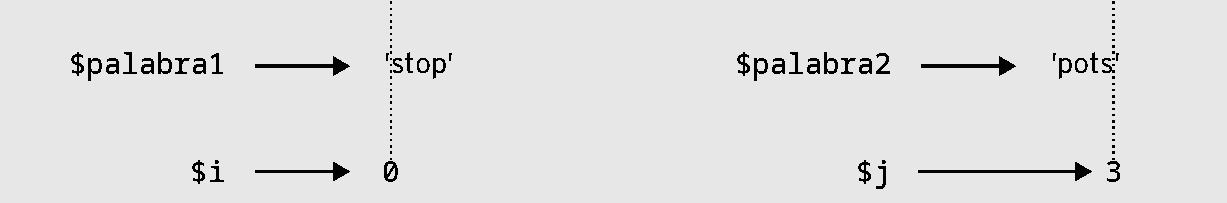
\includegraphics[scale=0.5]{figs/state6.pdf}}
\caption{State diagram.}
\label{fig.state4}
\end{figure}

We took some license by arranging the variables in the frame
and adding dotted lines to show that the values of {\tt \$i} 
and {\tt \$j} indicate characters in {\tt \$word1} and 
{\tt \$word2}.

Starting with this diagram, run the program on paper, changing 
the values of {\tt \$i} and {\tt \$j} during each iteration. 
Find and fix the second error in this function.

Solution: \ref{sol_isreverse}.
\label{isreverse}
\index{is-reverse}


\section{Glossary}

\begin{description}

\item[Object] Something a variable can store.  For now,
you can use ``object'' and ``value'' interchangeably.
\index{object}

\item[Sequence] An ordered collection of
values where each value is identified by an integer index.
\index{sequence}

\item[Item] One of the values in a sequence.
\index{item}

\item[Index] An integer value used to select an item in
a sequence, such as a character in a string.  In Perl
indices start from 0.
\index{index}

\item[Slice] A part of a string specified by a range of indices.
\index{slice}

\item[Empty string] A string with no characters and length 0, represented
by two quotation marks.
\index{empty string}

\item[Traverse] To iterate through the items in a sequence,
performing a similar operation on each.
\index{traversal}

\index{search}
\item[Search] A pattern of traversal that stops
when it finds what it is looking for.
\index{search!pattern}
\index{pattern!search}

\index{counter}
\item[Counter] A variable used to count something, usually initialized
to zero and then incremented.

\index{regular expression}
\item[Regular expressions] A computing sublanguage derived 
from the formal language theory.

\index{pattern}
\item[Pattern] A sequence of characters using a special 
syntax to describe from left to right the content that 
is intended to be matched within a target string.

\index{regex}
\item[Regexes] A pattern-matching sublanguage of Perl~6 
derived from regular expressions.

\index{backtracking}
\item[Backtracking] The process by which when a given attempt 
to match a string fails, the regex engine abandons part of 
the current match attempt, goes back into the string, and 
tries to see if it can find another route to a successful 
match. The backtracking process eventually stops as soon 
as a successful match succeeds, or ultimately when all 
possible match possibilities have failed.

\end{description}


\section{Exercises}


\begin{exercise}
\label{count_a}
\index{count method}
\index{method!count}
\index{index function}

Write a subroutine that uses the {\tt index} function in a 
loop to count the number of ``a'' characters in \verb"'banana'",
as we did in Section~\ref{counter}. Modify it to count 
any letter in any word passed as arguments to the subroutine.

Write another subroutine counting a given letter in a given 
word using the {\tt substr} function.
\index{substr function}

Solution: \ref{sol_count_a}
\end{exercise}


\begin{exercise}

\label{islower}
\index{lower case!character class}
\index{character class}
The \verb'<[a..z]>' character class matches any lower case 
character (only plain ASCII lower case characters, not 
Unicode characters). The following subroutine:

\begin{verbatim}[fontshape=up]
sub is-lower (Str $char) { 
    return so $char ~~ /^<[a..z]>$/
}
\end{verbatim}

should return {\tt True} if its argument is an ASCII lower case 
letter and {\tt False} otherwise. Test that it works as 
expected (and amend it if needed). The {\tt so} function 
coerces the result of the regex match into a Boolean value.

The following subroutines use the {\tt is-lower} subroutine 
and are all {\em intended} to check 
whether a string contains any lowercase letters, but at 
least some of them are wrong.  Analyze each subroutine by hand, 
determine whether it is correct, and describe what it 
actually does (assuming that the parameter is a string). Then 
test them with various input strings to check whether your 
analysis was correct.

\begin{verbatim}[fontshape=up]
# ATTENTION: some of the subroutines below are wrong

sub any_lowercase1(Str $string){
    for $string.comb -> $char {
        if is-lower $char {
            return True;
        } else {
            return False;
        }
    }
}

sub any_lowercase2(Str $string){
    for $string.comb -> $char {
        if is-lower "char" {
            return True;
        } else {
            return False;
        }
    }
}

sub any_lowercase3(Str $string){
    my $flag;
    for $string.comb -> $char {
        $flag =  is-lower $char;
    }
    return $flag;
}

sub any_lowercase4(Str $string){
    my $flag = False;
    for $string.comb -> $char {
        $flag = $flag or is-lower $char;
    }
    return $flag;
}

sub any_lowercase5(Str $string){
    my $flag = False;
    for $string.comb -> $char {
        if is-lower $char {
            $flag = True;
        }
    }
    return $flag;
}

sub any_lowercase6(Str $string){
    for $string.comb -> $char {
        if is-lower $char {
            return 'True';
        }
    }
    return 'False';
}

sub any_lowercase7(Str $string){
    for $string.comb -> $char {
        return True if is-lower $char;
    }
    return False;
}

sub any_lowercase8(Str $string){
    for $string.comb -> $char {
        return False unless is-lower $char;
    }
    return True;
}

sub any_lowercase9(Str $string){
    for $string.comb -> $char {
        if not is-lower $char {
            return False;
        }
    return True;
    }
}
\end{verbatim}

Solution: \ref{sol_islower}.

\end{exercise}


\begin{exercise}
\index{letter rotation}
\index{rotation, letter}
\index{Caesar cipher}

\label{rotate}
A Caesar cipher is a weak form of encryption that involves 
``rotating'' each letter by a fixed number of places.  To 
rotate a letter means to shift it through the alphabet, 
wrapping around to the beginning if necessary, so ``A'' 
rotated by 3 is ``D'' and ``Z'' rotated by 1 is ``A.''

To rotate a word, rotate each letter by the same amount.
For example, ``cheer'' rotated by 7 is ``jolly'' and ``melon'' rotated
by -10 is ``cubed.''  In the movie {\em 2001: A Space Odyssey}, the 
ship computer is called HAL, which is IBM rotated by -1.

Write a function called \verb"rotate-word"
that takes a string and an integer as parameters, and returns
a new string that contains the letters from the original string
rotated by the given amount.  

You might want to use the built-in functions {\tt ord}, which 
converts a character to a numeric code (Unicode code point), and 
{\tt chr}, which converts such numeric codes back to characters:
\index{ord function}
\index{chr function}
\index{function!ord}
\index{function!chr}

\begin{verbatim}[fontshape=up]
> say 'c'.ord;
99
> say chr 99
c
\end{verbatim}
%

Letters of the alphabet are encoded in alphabetical
order, so for example:
\index{alphabetic order}

\begin{verbatim}[fontshape=up]
> ord('c') - ord('a')
2
\end{verbatim}

because \verb"'c'" is the second letter after \verb"'a'" in 
the alphabet.  But beware: the numeric codes for upper case 
letters are different.
\index{upper case}
\index{case!upper}

\index{rot13}
Potentially offensive jokes on the internet are sometimes 
encoded in ROT13, which is a Caesar cipher with rotation 13. 
Since 13 is half the number of letters in our alphabet, 
applying rotation 13 twice returns the original word, 
so that the same procedure can be used for both encoding 
and decoding in rotation 13. If you are not
easily offended, find and decode some of these jokes. (ROT13 
is also used for other purposes, such as weakly hiding the 
solution to a puzzle.) 

Solution: \ref{sol_rotate}.

\end{exercise}

